\documentclass[10pt,letterpaper,unboxed,cm]{exam}
\usepackage[margin=1in]{geometry}
\usepackage{amsmath,mathabx}
\usepackage{color}
\usepackage{mdframed}
\usepackage{graphicx}
\usepackage{changepage}
\usepackage[skip=8pt]{parskip}
\usepackage{booktabs}



\begin{document}



% HEADER
\setlength{\parskip}{4pt}
\hfill{OpenIntro Statistics - 4th Edition}

\hfill{Chapter 1 Exercises}

\hfill{December 12, 2024}

\hfill{ODD SOLUTIONS}
\setlength{\parskip}{8pt}
\rule{\linewidth}{2pt}
% HEADER



\begin{questions}



% QUESTION 1
	\question \underline{1.1 Migraine and acupuncture, Part I.}

    A migraine is a particularly painful type of headache, which patients sometimes wish to treat with acupuncture. To determine whether acupuncture relieves migraine pain, researchers conducted a randomized controlled study where 89 females diagnosed with migraine headaches were randomly assigned to one of two groups: treatment or control. 43 patients in the treatment group received acupuncture that is specifically designed to treat migraines. 46 patients in the control group received placebo acupuncture (needle insertion at non-acupoint locations). 24 hours after patients received acupuncture, they were asked if they were pain free. Results are summarized in the contingency table below.

    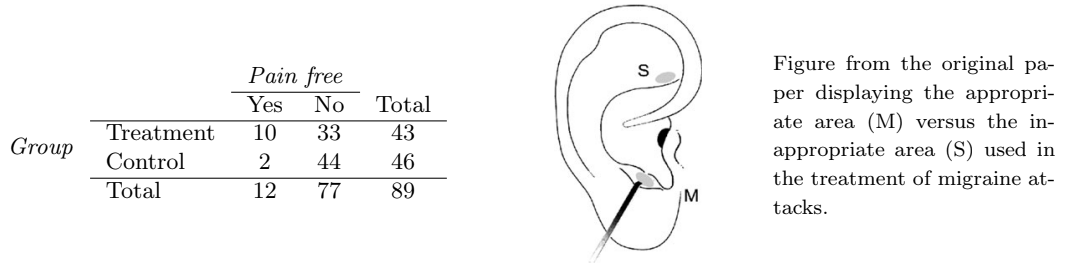
\includegraphics[width=\textwidth]{exercise1.1.png}
    
	\begin{parts}
		\part What percent of patients in the treatment group were pain free 24 hours after receiving acupuncture?
        
        \bigskip
        {\bf $10/43 \approx 0.23, ~~23\%$} 
        \bigskip

		\part What percent were pain free in the control group?
        
        \bigskip
        {\bf $2/46 \approx 0.04, ~~4\%$} 
        \bigskip

		\part In which group did a higher percent of patients become pain free 24 hours after receiving acupuncture?
        
        \bigskip
        {\bf The treatment group had a higher percent of patients becoming pain free at 23\% compared to the control group's 4\%.} 
        \bigskip

		\part Your findings so far might suggest that acupuncture is an effective treatment for migraines for all people who suffer from migraines. However, this is not the only possible conclusion that can be drawn based on your findings so far. What is one other possible explanation for the observed difference between the percentages of patients that are pain free 24 hours after receiving acupuncture in the two groups?
        
        \bigskip
        {\bf Patients from the treatment group may have tried other methods for alleviating their pain outside of the experiment, within 24 hours of receiving acupuncture.} 
        \bigskip

	\end{parts}
% QUESTION 1



% QUESTION 2
	\question \underline{1.3 Air pollution and birth outcomes, study components.}

    Researchers collected data to examine the relationship between air pollutants and preterm births in Southern California. During the study air pollution levels were measured by air quality monitoring stations. Specifically, levels of carbon monoxide were recorded in parts per million, nitrogen dioxide and ozone in parts per hundred million, and coarse particulate matter ($PM_{10}$) in $\mu g/m^3$. Length of gestation data were collected on 143,196 births between the years 1989 and 1993, and air pollution exposure during gestation was calculated for each birth. The analysis suggested that increased ambient $PM_{10}$ and, to a lesser degree, CO concentrations may be associated with the occurrence of preterm births
    
	\begin{parts}
		\part Identify the main research question of the study.
        
        \bigskip
        {\bf What is the impact of air pollution on preterm births in Southern California?} 
        \bigskip

		\part Who are the subjects in this study, and how many are included?
        
        \bigskip
        {\bf The subjects in this study were people giving birth in Southern California between the years 1989 and 1993. $143,196$ subjects were included.} 
        \bigskip

		\part What are the variables in the study? Identify each variable as numerical or categorical. If numerical, state whether the variable is discrete or continuous. If categorical, state whether the variable is ordinal.
        
        \bigskip
        {\bf 
        \begin{itemize}
            \item Length of gestation: numerical, continuous
            \item Date: categorical, ordinal
            \item Levels of carbon monoxide: numerical, continuous
            \item Levels of nitrogen dioxide: numerical, continuous
            \item Levels of ozone: numerical, continuous
            \item Levels of coarse particulate matter: numerical, continuous
        \end{itemize}
        } 
        \bigskip
	\end{parts}
% QUESTION 2



% QUESTION 3
	\question \underline{1.5 Cheaters, study components.}

    Researchers studying the relationship between honesty, age and self- control conducted an experiment on 160 children between the ages of 5 and 15. Participants reported their age, sex, and whether they were an only child or not. The researchers asked each child to toss a fair coin in private and to record the outcome (white or black) on a paper sheet, and said they would only reward children who report white. The study's findings can be summarized as follows: "Half the students were explicitly told not to cheat and the others were not given any explicit instructions. In the no instruction group probability of cheating was found to be uniform across groups based on child's characteristics. In the group that was explicitly told to not cheat, girls were less likely to cheat, and while rate of cheating didn't vary by age for boys, it decreased with age for girls."
    
	\begin{parts}
		\part Identify the main research question of the study.
        
        \bigskip
        {\bf Are levels of honesty and self-control related to ones age or gender?} 
        \bigskip

		\part Who are the subjects in this study, and how many are included?
        
        \bigskip
        {\bf The subjects include 160 children between the ages of 5 and 15.} 
        \bigskip

		\part How many variables were recorded for each subject in the study in order to conclude these findings? State the variables and their types.
        
        \bigskip
        {\bf 
        \begin{itemize}
            \item Age: numerical, discrete
            \item sex: categorical, nominal
            \item Only child: categorical, nominal
            \item Given explicit instructions: categorical, nominal
            \item Toss result: categorical, nominal
            \item Cheated: categorical, nominal
        \end{itemize}
        } 
        \bigskip
	\end{parts}
% QUESTION 3



% QUESTION 4
	\question \underline{1.7 Migraine and acupuncture, Part II.}

    Exercise 1.1 introduced a study exploring whether acupuncture had any effect on migraines. Researchers conducted a randomized controlled study where patients were randomly assigned to one of two groups: treatment or control. The patients in the treatment group received acupuncture that was specifically designed to treat migraines. The patients in the control group received placebo acupuncture (needle insertion at non-acupoint locations). 24 hours after patients received acupuncture, they were asked if they were pain free. What are the explanatory and response variables in
    this study?
    
    \bigskip
        {\bf 
        \begin{itemize}
            \item Explanatory: Acupuncture insertion location
            \item Response: Migraine persistence after 24 hours
        \end{itemize}
        } 
    \bigskip
% QUESTION 4



% QUESTION 5
	\question \underline{1.9 Fisher’s irises.} 

    Sir Ronald Aylmer Fisher was an English statistician, evolutionary biologist, and geneticist who worked on a data set that contained sepal length and width, and petal length and width from three species of iris flowers ({\it setosa, versicolor and virginica}). There were 50 flowers from each species in the data set.
    
	\begin{parts}
		\part How many cases were included in the data?
        
        \bigskip
        {\bf $50$ flowers from $3$ different species creates $150$ cases in the data.} 
        \bigskip

		\part How many numerical variables are included in the data? Indicate what they are, and if they are continuous or discrete.
        
        \bigskip
        {\bf 
        \begin{itemize}
            \item Sepal length: continuous
            \item Sepal width: continuous
            \item Petal length: continuous
            \item Petal width: continuous
        \end{itemize}
        } 
        \bigskip

		\part How many categorical variables are included in the data, and what are they? List the corresponding levels (categories).
        
        {\bf There is $1$ nominal categorical variable in this data: species. The levels include setosa, versicolor and virginica.} 
        \bigskip
	\end{parts}
% QUESTION 5



% QUESTION 6
	\question \underline{1.11 US Airports.}

    The visualization below shows the geographical distribution of airports in the contiguous United States and Washington, DC. This visualization was constructed based on a dataset where each observation is an airport.

    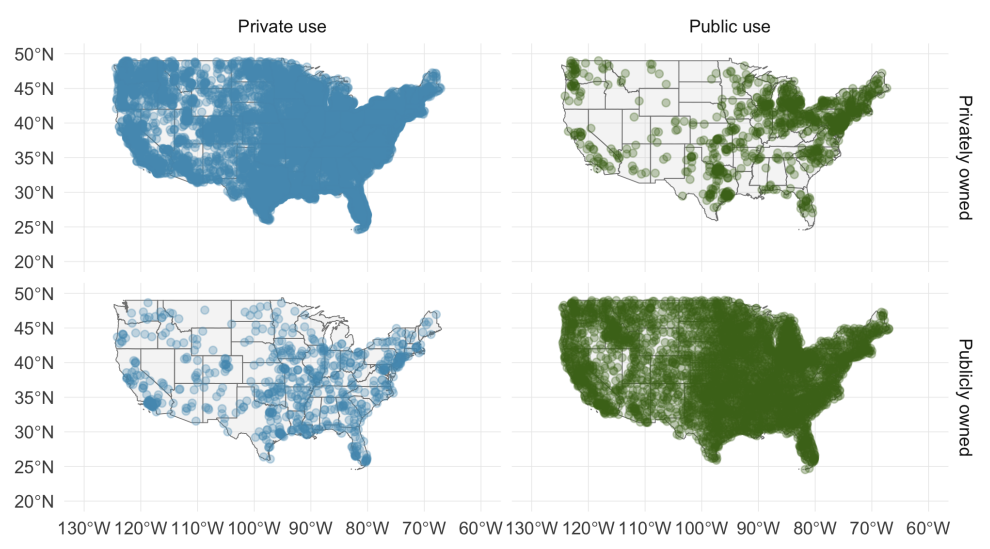
\includegraphics[width=\textwidth]{usmap.png}
    
	\begin{parts}
		\part List the variables used in creating this visualization.
        
        \bigskip
        {\bf 
        \begin{itemize}
            \item Longitude
            \item Latitude
            \item Use by
            \item Owned by
        \end{itemize}
        }
        \bigskip

		\part Indicate whether each variable in the study is numerical or categorical. If numerical, identify as continuous or discrete. If categorical, indicate if the variable is ordinal.
        
        \bigskip
        {\bf 
        \begin{itemize}
            \item Longitude: numerical, continuous 
            \item Latitude: numerical, continuous
            \item Use by: categorical, nominal
            \item Owned by: categorical, nominal
        \end{itemize}
        }
        \bigskip
	\end{parts}
% QUESTION 6



% QUESTION 7
	\question \underline{1.13 Air pollution and birth outcomes, scope of inference.}

    Exercise 1.3 introduces a study where researchers collected data to examine the relationship between air pollutants and preterm births in Southern California. During the study air pollution levels were measured by air quality monitoring stations. Length of gestation data were collected on 143,196 births between the years 1989 and 1993, and air pollution exposure during gestation was calculated for each birth.
    
	\begin{parts}
		\part Identify the population of interest and the sample in this study.
        
        \bigskip
        {\bf The population of interest is of all people who gave birth in Southern California between the years 1989 and 1993. The sample are the $143,196$ births collected.} 
        \bigskip

		\part Comment on whether or not the results of the study can be generalized to the population, and if the findings of the study can be used to establish causal relationships.
        
        \bigskip
        {\bf The sample size of this study is large enough to conclude that the results can be generalized to the population of births in Southern California. However, since this was an observational study we could not determine any causal relationships between the two factors being analyzed.} 
        \bigskip
	\end{parts}
% QUESTION 7



% QUESTION 8
	\question \underline{1.15 Buteyko method, scope of inference.}

    Exercise 1.4 introduces a study on using the Buteyko shallow breathing technique to reduce asthma symptoms and improve quality of life. As part of this study 600 asthma patients aged 18-69 who relied on medication for asthma treatment were recruited and randomly assigned to two groups: one practiced the Buteyko method and the other did not. Those in the Buteyko group experienced, on average, a significant reduction in asthma symptoms and an improvement in quality of life.
    
	\begin{parts}
		\part Identify the population of interest and the sample in this study.
        
        \bigskip
        {\bf The population of interest are people who experience symptoms of asthma. The sample includes asthma patients aged 18-69 who relied on medication for asthma treatment.} 
        \bigskip

		\part Comment on whether or not the results of the study can be generalized to the population, and if the findings of the study can be used to establish causal relationships.
        
        \bigskip
        {\bf Because of the relatively small size of the sample size, my confidence in the results representing the whole population of interest in not strong. However, this result was found through an experiment with randomly selected groups which infers a causal relationship between the Butkeyko method and asthma symptons/improve in Q.O.L.} 
        \bigskip
	\end{parts}
% QUESTION 8



% QUESTION 9
	\question \underline{1.17 Relaxing after work.}

    The General Social Survey asked the question, “After an average work day, about how many hours do you have to relax or pursue activities that you enjoy?” to a random sample of 1,155 Americans. The average relaxing time was found to be 1.65 hours. Determine which of the following is an observation, a variable, a sample statistic (value calculated based on the observed sample), or a population parameter.
    
	\begin{parts}
		\part An American in the sample.
        
        \bigskip
        {\bf Observation} 
        \bigskip

		\part Number of hours spent relaxing after an average work day.
        
        \bigskip
        {\bf Variable} 
        \bigskip

		\part 1.65.
        
        \bigskip
        {\bf Sample statistic} 
        \bigskip

		\part Average number of hours all Americans spend relaxing after an average work day.
        
        \bigskip
        {\bf Population parameter} 
        \bigskip

	\end{parts}
% QUESTION 9



% QUESTION 10
	\question \underline{1.19 Course satisfaction across sections.}

    A large college class has 160 students. All 160 students attend the lectures together, but the students are divided into 4 groups, each of 40 students, for lab sections administered by different teaching assistants. The professor wants to conduct a survey about how satisfied the students are with the course, and he believes that the lab section a student is in might affect the student’s overall satisfaction with the course.
    
	\begin{parts}
		\part What type of study is this?
        
        \bigskip
        {\bf This study is an observational study since the data is being collected through the students' existing environments without interference.} 
        \bigskip

		\part Suggest a sampling strategy for carrying out this study.
        
        \bigskip
        {\bf Since all students share the same lecture and we can safely assume they are all of similar ages, using a stratified sampling technique may be useful. Each lab section can represent a strata.} 
        \bigskip
	\end{parts}
% QUESTION 10



% QUESTION 11
	\question \underline{1.21 Internet use and life expectancy.}

    The following scatterplot was created as part of a study evaluating the relationship between estimated life expectancy at birth (as of 2014) and percentage of internet users (as of 2009) in 208 countries for which such data were available.

    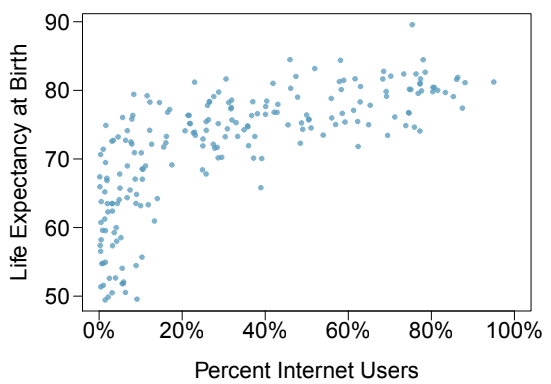
\includegraphics[width=0.5\textwidth]{internetscatter.png}
    
	\begin{parts}
		\part Describe the relationship between life expectancy and percentage of internet users.
        
        \bigskip
        {\bf There is a positive correlation between these two variables.} 
        \bigskip

		\part What type of study is this?
        
        \bigskip
        {\bf This study is observational because it collected its data from past records from different countries.} 
        \bigskip

		\part State a possible confounding variable that might explain this relationship and describe its potential effect.
        
        \bigskip
        {\bf One possible confounding variable might be country GDP since the use of internet requires access to devices and infrastructure supporting an internet connection.} 
        \bigskip
	\end{parts}
% QUESTION 11



% QUESTION 12
	\question \underline{1.23 Evaluate sampling methods.}

    A university wants to determine what fraction of its undergraduate student body support a new \$25 annual fee to improve the student union. For each proposed method below, indicate whether the method is reasonable or not.
    
	\begin{parts}
		\part Survey a simple random sample of 500 students.
        
        \bigskip
        {\bf This method may not be reasonable for two reasons. A simple random sample may have a convenience bias. The relatively small sample size of students also may not accurately reflect the entire population's opinion.} 
        \bigskip

		\part Stratify students by their field of study, then sample 10\% of students from each stratum.
        
        \bigskip
        {\bf This method could work well. Using field of study as the variable to create each strata is easy to do and generalizes across the entire university. One concern may be that the number of students enrolled into each field of study may be skewed.} 
        \bigskip

		\part Cluster students by their ages (e.g. 18 years old in one cluster, 19 years old in one cluster, etc.), then randomly sample three clusters and survey all students in those clusters.
        
        \bigskip
        {\bf This may not work well since there are only a small handful of skewed clusters that can be created. Using this method might lead the same to completely ignore relevant groups of students such as freshman or seniors.} 
        \bigskip
	\end{parts}
% QUESTION 12



% QUESTION 13
	\question \underline{1.25 Haters are gonna hate, study confirms.}

    A study published in the {\it Journal of Personality and Social Psychology} asked a group of 200 randomly sampled men and women to evaluate how they felt about various subjects, such as camping, health care, architecture, taxidermy, crossword puzzles, and Japan in order to measure their attitude towards mostly independent stimuli. Then, they presented the participants with information about a new product: a microwave oven. This microwave oven does not exist, but the participants didn’t know this, and were given three positive and three negative fake reviews. People who reacted positively to the subjects on the dispositional attitude measurement also tended to react positively to the microwave oven, and those who reacted negatively tended to react negatively to it. Researchers concluded that “some people tend to like things, whereas others tend to dislike things, and a more thorough understanding of this tendency will lead to a more thorough understanding of the psychology of attitudes.”
    
	\begin{parts}
		\part What are the cases?
        
        \bigskip
        {\bf Each of the 200 individuals randomly sampled are cases.} 
        \bigskip

		\part What is (are) the response variable(s) in this study?
        
        \bigskip
        {\bf The reaction to the microwave.} 
        \bigskip

		\part What is (are) the explanatory variable(s) in this study?
        
        \bigskip
        {\bf The reaction to the subjects on the dispositional attitude.} 
        \bigskip

		\part Does the study employ random sampling?
        
        \bigskip
        {\bf Yes.} 
        \bigskip

		\part Is this an observational study or an experiment? Explain your reasoning.
        
        \bigskip
        {\bf This study is an observational study because the data this study collects are observations of each individuals dispositional attitude without any interference. The response variable was not collected randomly as each individual received the same number of positive and negative reviews, so the design of this study was not experimental.} 
        \bigskip

		\part Can we establish a causal link between the explanatory and response variables?
        
        \bigskip
        {\bf No, since this was an observational study the results cannot infer a causal link between each variable.} 
        \bigskip

		\part Can the results of the study be generalized to the population at large?
        
        \bigskip
        {\bf No. A sample size of 200 is extremely small relative to the population of even a single city. The paragraph does not specify where the samples were collected from or what the population of interest is.} 
        \bigskip

	\end{parts}
% QUESTION 13



% QUESTION 14
	\question \underline{1.27 Sampling strategies.}

    A statistics student who is curious about the relationship between the amount of time students spend on social networking sites and their performance at school decides to conduct a survey. Various research strategies for collecting data are described below. In each, name the sampling method proposed and any bias you might expect.
    
	\begin{parts}
		\part He randomly samples 40 students from the study’s population, gives them the survey, asks them to fill it out and bring it back the next day.
        
        \bigskip
        {\bf Simple random sampling; non-response bias} 
        \bigskip

		\part He gives out the survey only to his friends, making sure each one of them fills out the survey.
        
        \bigskip
        {\bf Cluster sampling; convenience bias} 
        \bigskip

		\part He posts a link to an online survey on Facebook and asks his friends to fill out the survey.
        
        \bigskip
        {\bf Multistage sampling; convenience and non-response bias} 
        \bigskip

		\part He randomly samples 5 classes and asks a random sample of students from those classes to fill out the survey.
        
        \bigskip
        {\bf Multistage sampling; convenience bias} 
        \bigskip

	\end{parts}
% QUESTION 14



% QUESTION 15
	\question \underline{1.29 Light and exam performance.}

    A study is designed to test the effect of light level on exam performance of students. The researcher believes that light levels might have different effects on males and females, so wants to make sure both are equally represented in each treatment. The treatments are fluorescent overhead lighting, yellow overhead lighting, no overhead lighting (only desk lamps).
    
	\begin{parts}
		\part What is the response variable?
        
        \bigskip
        {\bf Exam performance of students} 
        \bigskip

		\part What is the explanatory variable? What are its levels?
        
        \bigskip
        {\bf Light levels; fluorescent overhead lighting, yellow overhead lighting, and no overhead lighting (only desk lamps)} 
        \bigskip

		\part What is the blocking variable? What are its levels?
        
        \bigskip
        {\bf The blocking variable is sex; female and male} 
        \bigskip
	\end{parts}
% QUESTION 15



% QUESTION 16
	\question \underline{1.31 Light, noise, and exam performance.}

    A study is designed to test the effect of light level and noise level on exam performance of students. The researcher believes that light and noise levels might have different effects on males and females, so wants to make sure both are equally represented in each treatment. The light treatments considered are fluorescent overhead lighting, yellow overhead lighting, no overhead lighting (only desk lamps). The noise treatments considered are no noise, construction noise, and human chatter noise.
    
	\begin{parts}
		\part What type of study is this?
        
        \bigskip
        {\bf This is an experimental study since the study is designed by strategically controlling explanatory variables such as noise and measuring responses from groups.} 
        \bigskip

		\part How many factors are considered in this study? Identify them, and describe their levels.
        
        \bigskip
        {\bf 
        \begin{itemize}
            \item Sex: male, female
            \item Light level: fluorescent overhead lighting, yellow overhead lighting, and no overhead lighting (only desk lamps)
            \item Noise level: no noise, construction noise, and human chatter noise
        \end{itemize}
        }
        \bigskip

		\part What is the role of the sex variable in this study?
        
        \bigskip
        {\bf Sex is the blocking variable in this study because the researcher believes the explanatory variables may affect males and females differently which cannot be controlled.} 
        \bigskip
	\end{parts}
% QUESTION 16



% QUESTION 17
	\question \underline{1.33 Soda preference.}

    You would like to conduct an experiment in class to see if your classmates prefer the taste of regular Coke or Diet Coke. Briefly outline a design for this study.
    
    \bigskip
    {\bf Since the population is classmates in my class, I would employ simple random sampling on the class to collect the sample. This is an observational study so I would simply need to ask whether the sampled classmates prefer Coke or Diet Coke and record the responses. Explanatory variables might include age, sex, and major.} 
    \bigskip
% QUESTION 17



\end{questions}
\end{document}